\chapter{导波与谐振腔}\label{ch:b2:guided-waves}

雷达的脉冲在矩形铜管内，
从发射机传到天线盘；网络连接的光在比头发还细的玻璃丝中
传播一万千米；烤箱里的微波
在其内壁之间来回反射，并形成
冷热相间的分布。被导体或折射壁限制的波
不再是可以自由传播到任何地方的平面波：它必须
满足壁面上的边界条件，这决定了它可能取的形状——
即\emph{模式}——，并禁止它在低于某一
\emph{截止频率}时存在。本章先构造最简单的导波结构，
即两块平行导体板，它由
\cref{ch:b2:wave-interfaces}中的反射得到；随后讨论矩形波导、
闭合谐振腔，以及从射线的角度看的光纤。

\section{两导体平板之间的波}

\begin{proposition}[平行板导波的模式]\label{prop:b2:guided-waves:plates}
\index{波导}\index{导波}\index{模式（波导）}\index{截止频率（波导）}
两个\omterm{prop:b2:wave-interfaces:conductors}{理想导体}平面 $y = 0$ 与 $y = a$ 围成真空区域。
寻找沿 $z$ 方向传播的波，其 $\vect E = E(y)\,\eu^{\iu(\omega t - k_gz)}
\vect e_x$（电场平行于平板，垂直于
传播方向）。真空中的\omterm{thm:b2:maxwell-equations:maxwell}{麦克斯韦方程组}及平板上 $E = 0$ 的条件
给出如下结果：
\[
E(y) = E_0\sin\frac{n\pi y}a , \qquad
k_g^2 = \frac{\omega^2}{c^2} - \Bigl(\frac{n\pi}a\Bigr)^2 , \qquad n = 1, 2, \dots
\]
模式 $n$ 仅在高于其\emph{截止频率} $f_n = nc/2a$ 时才能传播；
低于该频率时，$k_g$ 为虚数，场沿导波方向衰减。
其\omterm{def:b2:dispersion-wave-packets:relation}{相速度}与\omterm{prop:b2:dispersion-wave-packets:group}{群速度}为
\[
v_\varphi = \frac c{\sqrt{1 - f_n^2/f^2}} > c , \qquad
v_g = c\sqrt{1 - f_n^2/f^2} < c , \qquad v_\varphi v_g = c^2 ,
\]
其磁场在 $y$ 方向和 $z$ 方向上都有分量：导波
在传播方向上不是横波。
\end{proposition}

\begin{proof}
代入 $\Delta\vect E = \partial_t^2\vect E/c^2$，得 $E'' - k_g^2E = -(\omega^2/c^2)E$，即
$E'' + (\omega^2/c^2 - k_g^2)E = 0$，其在 $y = 0$ 与
$y = a$ 处取零值的解为正弦函数，且 $\omega^2/c^2 - k_g^2 = (n\pi/a)^2$；$\operatorname{div}
\vect E = 0$ 成立，因为 $E_x$ 不依赖于 $x$。由法拉第定律得
$\underline B_y = (k_g/\omega)\underline E$，$\underline B_z = (\iu/\omega)\partial_y\underline E$，后者
与前者相位正交。速度由\omterm{def:b2:dispersion-wave-packets:relation}{色散关系}的克莱因–戈登形式导出
（\cref{ch:b2:dispersion-wave-packets}）。
\end{proof}

\begin{remark}[作为两列平面波的模式]\label{rem:b2:guided-waves:zigzag}
$\sin(n\pi y/a)\eu^{-\iu k_gz}$ 是两列平面波之和，二者的波矢为
$(0, \pm n\pi/a, k_g)$，模长为 $\omega/c$，它们在两板之间来回反射，
与轴成角 $\theta$，且 $\cos\theta = k_gc/\omega$：
导模是一列在两壁之间呈之字形传播的平面波，每次在壁上以
$r = -1$ 反射，横向驻波
即它与自身相干相长的条件。能量
沿之字形以速率 $c$ 传播，因此沿轴的速度为 $c\cos\theta = v_g$；
波峰与轴的交点运动的速度为 $c/\cos\theta = v_\varphi$。在
截止处，波在两板之间来回反射，
不沿导波方向前进。
\end{remark}

\begin{omfigure}
\begin{tikzpicture}[font=\small, x=1cm, y=1cm, >=Stealth]
  \begin{scope}
    \draw[thick] (-3,0) -- (3,0); \draw[thick] (-3,2) -- (3,2);
    \fill[pattern=north east lines] (-3,-0.15) rectangle (3,0); \fill[pattern=north east lines] (-3,2) rectangle (3,2.15);
    \draw[omDef, thick, ->] (-2.8,0.2) -- (-1.6,1.8); \draw[omDef, thick, ->] (-1.6,1.8) -- (-0.4,0.2); \draw[omDef, thick, ->] (-0.4,0.2) -- (0.8,1.8); \draw[omDef, thick, ->] (0.8,1.8) -- (2.0,0.2); \draw[omDef, thick, ->] (2.0,0.2) -- (2.8,1.27);
    \draw (-0.4,0.2) -- (0.6,0.2); \draw (0.3,0.2) arc[start angle=0, end angle=53, radius=0.7]; \node[font=\footnotesize] at (0.75,0.55) {$\theta$};
    \draw[->, thick] (-3,-0.6) -- (3,-0.6) node[right, font=\footnotesize] {$z$};
    \node[font=\footnotesize] at (-3.3,1) {$a$};
    \draw[<->] (-3.15,0) -- (-3.15,2);
  \end{scope}
  \begin{scope}[xshift=8.4cm]
    \draw[thick] (0,0) -- (0,2); \draw[thick] (3.6,0) -- (3.6,2);
    \fill[pattern=north east lines] (-0.15,0) rectangle (0,2); \fill[pattern=north east lines] (3.6,0) rectangle (3.75,2);
    \draw[omThm, thick, domain=0:3.6, samples=50] plot (\x,{1+0.8*sin(50*\x)});
    \draw[omProp, thick, domain=0:3.6, samples=50] plot (\x,{1+0.6*sin(100*\x)});
    \draw[dashed] (0,1) -- (3.6,1);
    \node[omThm, font=\footnotesize] at (1.8,2.3) {$n = 1$}; \node[omProp, font=\footnotesize] at (0.9,1.9) {$n = 2$};
    \draw[<->] (0,-0.3) -- (3.6,-0.3) node[midway, below, font=\footnotesize] {$a$（$y$ 轴）};
  \end{scope}
\end{tikzpicture}

{\small 左：导模是一列在两平板之间来回反射的平面波；
频率趋近截止频率时，角 $\theta$ 增大。
右：前两个模式的横向分布 $E(y)$，
在导体壁上为零。}
\end{omfigure}

\begin{omfigure}
\begin{tikzpicture}
\begin{axis}[omaxis, axis x line=bottom, axis y line=left, width=6.6cm, height=4.8cm,
    xlabel={$k_g$}, ylabel={$\omega$}, xmin=0, xmax=3, ymin=0, ymax=4, xtick=\empty, ytick={1,2,3}, yticklabels={$\omega_1$, $\omega_2$, $\omega_3$}, samples=80,
    xlabel style={at={(axis description cs:1.0,0.0)}, anchor=west},
    ylabel style={at={(axis description cs:0.0,1.0)}, anchor=south}]
  \addplot[omThm, thick, domain=0:3] {sqrt(1+x*x)};
  \addplot[omThm, thick, domain=0:3] {sqrt(4+x*x)};
  \addplot[omThm, thick, domain=0:3] {sqrt(9+x*x)};
  \addplot[omDef, dashed, domain=0:3] {x};
  \node[font=\scriptsize, anchor=west] at (axis cs:2.2,2.05) {$\omega = ck_g$};
\end{axis}
\end{tikzpicture}
\hfill
\begin{tikzpicture}
\begin{axis}[omaxis, axis x line=bottom, axis y line=left, width=6.6cm, height=4.8cm,
    xlabel={$f/f_1$}, ylabel={$v/c$}, xmin=1, xmax=4, ymin=0, ymax=2.5, xtick={1,2,3,4}, ytick={1}, samples=100,
    xlabel style={at={(axis description cs:0.5,-0.12)}, anchor=north},
    ylabel style={at={(axis description cs:-0.1,0.5)}, rotate=90, anchor=south},
    legend style={font=\scriptsize, at={(0.97,0.95)}, anchor=north east, draw=none, fill=none}]
  \addplot[omThm, thick, domain=1.05:4] {1/sqrt(1-1/(x*x))};
  \addplot[omDef, thick, domain=1:4] {sqrt(1-1/(x*x))};
  \addplot[black, dashed, domain=1:4] {1};
  \legend{$v_\varphi$, $v_g$}
\end{axis}
\end{tikzpicture}

{\small 左：导波管前三个模式的色散曲线，
每条都是从其截止频率出发的双曲线。右：某一模式的\omterm{def:b2:dispersion-wave-packets:relation}{相速度}和\omterm{prop:b2:dispersion-wave-packets:group}{群速度}随频率的变化；
能量在截止频率附近缓慢
爬行，远高于截止频率时趋近 $c$。}
\end{omfigure}

\begin{example}[数值]\label{ex:b2:guided-waves:numbers}
两板相距 \qty{3}{cm}，$f_1 = \qty{5}{GHz}$，$f_2 = \qty{10}{GHz}$；在这两个频率之间
只有一个模式能够传播（\emph{单模}
运行方式，它使脉冲不会分裂为若干个
具有不同 $v_g$ 的脉冲）。在 \qty{8}{GHz} 时，模式 $n = 1$ 的 $v_g = 0.78c$，$v_\varphi =
1.28c$，导波波长 $\lambda_g = 2\pi/k_g = \qty{4.8}{cm}$，而非
自由空间中的 \qty{3.75}{cm}。在 \qty{4}{GHz} 时没有波能通过，场
按 $\eu^{-z/\ell}$ 衰减，其中 $\ell = c/2\pi\sqrt{f_1^2 - f^2} = \qty{1.6}{cm}$——
烤箱门网孔的原理，截止以下用作标定衰减器的导波管
的原理，以及通风用金属管道
的原理，它能让空气通过而挡住无线电波。
\end{example}

\section{矩形导波管与谐振腔}

\begin{proposition}[矩形导波管；TE$_{10}$ 模式]\label{prop:b2:guided-waves:rectangular}
\index{矩形导波管}\index{TE 模式}
截面为矩形、尺寸 $a \times b$（$a > b$）的空心金属管可传播
截止频率为下式的各模式：
\[
f_{mn} = \frac c2\sqrt{\Bigl(\frac ma\Bigr)^2 + \Bigl(\frac nb\Bigr)^2} ;
\]
最低模式即\emph{TE$_{10}$ 模式}（$f_{10} = c/2a$），其电场为 $\vect E = E_0\sin
(\pi x/a)\,\eu^{\iu(\omega t - k_gz)}\,\vect e_y$：沿宽边为一个半正弦，
沿窄边均匀，在两侧壁 $x = 0$、
$x = a$ 处为零——正是平行板模式，侧壁 $y = 0$、$b$
与 $\vect E$ 垂直，对其不起约束作用。该导波管
在 $f_{10}$ 与下一截止频率之间使用；其磁感线
在 $xz$ 平面内闭合，它们在管壁中感应出的电流
正是缝隙不能切断的。所传输的功率为 $\tfrac14\varepsilon_0cE_0^2\,ab
\sqrt{1 - f_{10}^2/f^2}$。
\end{proposition}

\begin{proof}
一般模式是 $\cos$/$\sin$ 在 $x$ 与 $y$ 方向上的乘积，并满足
四个壁面上的边界条件，由此得 $k_g^2 = \omega^2/c^2 - (m\pi/a)^2
- (n\pi/b)^2$（一般情形在本阶段不加证明地承认；TE$_{10}$ 情形即
上文命题）。功率：沿 $z$ 方向的平均\omterm{thm:b2:poynting-vector:poynting}{坡印廷矢量}为 $E_0^2\sin^2(\pi x/a)
\,k_g/2\mu_0\omega$ 在截面上积分。
\end{proof}

\begin{omfigure}
\begin{tikzpicture}[font=\small, x=1cm, y=1cm, >=Stealth]
  \begin{scope}
    \draw[thick] (0,0) rectangle (3.6,1.8);
    \foreach \x in {0.45,0.9,...,3.15} {
      \pgfmathsetmacro{\h}{0.75*sin(deg(180*\x/3.6))}
      \draw[omDef, ->] (\x,{0.9-\h}) -- (\x,{0.9+\h});
    }
    \node[font=\footnotesize] at (1.8,-0.35) {$a$}; \node[font=\footnotesize] at (-0.3,0.9) {$b$};
    \node[omDef, font=\footnotesize] at (1.8,2.15) {TE$_{10}$：$\vect E$ 沿窄边};
  \end{scope}
  \begin{scope}[xshift=7.0cm]
    \draw[thick] (0,0) rectangle (4.8,1.8);
    \draw[omProp, thick, postaction={decorate, decoration={markings, mark=at position 0.2 with {\arrow{>}}, mark=at position 0.7 with {\arrow{>}}}}] (1.2,0.9) ellipse (0.9 and 0.55);
    \draw[omProp, thick, postaction={decorate, decoration={markings, mark=at position 0.2 with {\arrow{<}}, mark=at position 0.7 with {\arrow{<}}}}] (3.6,0.9) ellipse (0.9 and 0.55);
    \node[omProp, font=\footnotesize] at (2.4,2.15) {$\vect B$ 在 $xz$ 平面内成环（俯视）};
    \draw[->, thick] (0,-0.85) -- (1.2,-0.85) node[right, font=\footnotesize] {$z$};
    \draw[<->] (0,-0.3) -- (2.4,-0.3) node[midway, below, font=\footnotesize] {$\lambda_g/2$};
  \end{scope}
\end{tikzpicture}

{\small \omterm{prop:b2:guided-waves:rectangular}{矩形导波管}的 TE$_{10}$ 模式：电场
沿窄边方向分布，沿宽边呈半正弦分布；
磁场在宽面所在平面内成环闭合，
其长为半个导波波长。}
\end{omfigure}

\begin{proposition}[谐振腔]\label{prop:b2:guided-waves:cavity}
\index{谐振腔}\index{模式（谐振腔）}
用相距 $d$ 的两块导体壁封闭导波管，即可将其
变为\emph{谐振腔}，其中导行波沿 $z$ 方向也须形成
驻波，$k_g = p\pi/d$；尺寸为
$a \times b \times d$ 的矩形盒的共振频率为
\[
f_{mnp} = \frac c2\sqrt{\Bigl(\frac ma\Bigr)^2 + \Bigl(\frac nb\Bigr)^2 + \Bigl(\frac pd\Bigr)^2} .
\]
频率低于 $f$ 的模式数按 $8\pi V f^3/3c^3$ 增长，
对体积为 $V$ 的盒子（在本阶段不加证明地承认：数一数格点
$(m/2a, n/2b, p/2d)$ 落在球的八分之一内的个数，并计入两种偏振）
——即热辐射理论将要用到的模式密度
（见\cref{ch:b2:thermal-radiation}）。每个模式都有品质因数
$Q$，由壁面损耗决定（表面电阻见
\cref{ch:b2:waves-in-media}），微波频率下铜腔的典型值为 $10^3$--$10^4$，
超导腔则为 $10^{10}$。
\end{proposition}

\begin{proof}
三个方向上的驻波，在六个壁面上形成波节；
波矢 $(m\pi/a, n\pi/b, p\pi/d)$ 的模为 $\omega/c$。
\end{proof}

\begin{example}[烤箱、雷达、时钟]\label{ex:b2:guided-waves:cavities}
尺寸为 $30 \times 30 \times 20$ cm$^3$ 的微波炉在 \qty{2.45}{GHz} 附近，
在磁控管频率的几个百分点之内有几十个模式：
场是驻波的叠加，其极大值
相距 \qty{6}{cm}，经转盘（以及“模式搅拌器”）
的作用而被抹平。雷达的磁控管本身即是一个谐振腔；粒子
加速器是一串超导腔，其 TM 模式
推动粒子束团；铯原子钟中的原子穿过一个微波
谐振腔，该腔调谐于 \qty{9.19}{GHz}。
\end{example}

\section{射线图景中的光纤}

\begin{proposition}[阶跃折射率光纤]\label{prop:b2:guided-waves:fibre}
\index{光纤}\index{数值孔径}\index{模式色散}
折射率为 $n_1$ 的玻璃纤芯外包一层折射率略低的
包层（折射率 $n_2$），光在纤芯边界处通过\omterm{thm:b2:wave-interfaces:snell}{全反射}被导引。
从空气射入端面、与轴线夹角为 $\alpha$ 的光线，
若 $\sin\alpha < \sqrt{n_1^2 - n_2^2}$，则光线被束缚，此量称为\emph{\omterm{prop:b2:guided-waves:fibre}{数值
孔径}}；不同角度的光线走过的路程不同，因而
长为 $L$ 的光纤中入射的脉冲会被展宽，展宽量为
\[
\Delta t = \frac{n_1L}c\Bigl(\frac{n_1}{n_2} - 1\Bigr) ,
\]
\emph{\omterm{prop:b2:guided-waves:fibre}{模式色散}}——对于 $n_1
- n_2 = 0.01$，每千米约 \qty{50}{ns}，多模光纤在十千米上仅能传输
每秒几兆比特。\emph{单模光纤}的纤芯
很细（\qty{9}{\micro m}），只有一个模式能够传播，
正如导波处于前两个截止频率之间时那样；剩下的是玻璃的
色度色散（见\cref{ch:b2:dispersion-wave-packets}）。
\end{proposition}

\begin{proof}
纤芯与包层界面处的\omterm{thm:b2:wave-interfaces:snell}{全反射}要求 $\sin\theta >
n_2/n_1$，其中 $\theta$ 为与界面法线的夹角；即 $\cos
\theta' > n_2/n_1$，其中 $\theta'$ 为纤内光线与轴线的夹角；
端面处的折射给出 $\sin\alpha = n_1\sin\theta'$，从而 $\sin\alpha < n_1\sqrt{1
- n_2^2/n_1^2}$。与轴线夹角最大的被束缚光线，走过的路程为 $L/\cos\theta' = Ln_1/n_2$
相比之下轴向光线走过 $L$，速率为 $c/n_1$。
\end{proof}

\begin{omfigure}
\begin{tikzpicture}[font=\small, x=1cm, y=1cm, >=Stealth]
  \fill[omDef!10] (-3.5,-1.0) rectangle (3.5,1.0);
  \fill[omDef!30] (-3.5,-0.5) rectangle (3.5,0.5);
  \draw[thick] (-3.5,0.5) -- (3.5,0.5) (-3.5,-0.5) -- (3.5,-0.5);
  \draw[omThm, thick, ->] (-4.6,-0.9) -- (-3.5,-0.35);
  \draw[omThm, thick] (-3.5,-0.35) -- (-2.3,0.5) -- (-0.9,-0.5) -- (0.5,0.5) -- (1.9,-0.5) -- (3.3,0.5);
  \draw[omProp, thick, ->] (-4.6,0) -- (3.4,0);
  \draw[dashed] (-3.5,-1.3) -- (-3.5,1.3);
  \node[font=\footnotesize] at (-4.3,-0.25) {$\alpha$};
  \node[font=\footnotesize] at (2.6,0.8) {包层 $n_2$}; \node[font=\footnotesize] at (2.6,0.2) {纤芯 $n_1$};
  \node[font=\footnotesize] at (0,-1.4) {$\sin\alpha < \sqrt{n_1^2 - n_2^2}$：被全反射束缚};
\end{tikzpicture}

{\small 射线图景中的阶跃折射率光纤：接收锥内的光线
经\omterm{thm:b2:wave-interfaces:snell}{全反射}被束缚；折线形的光线
到达时间晚于轴向光线——即\omterm{prop:b2:guided-waves:fibre}{模式色散}。}
\end{omfigure}

\begin{method}[导波问题的计算步骤]\label{met:b2:guided-waves:method}
(1) 确定管壁及其边界条件（导体上切向 $\vect E = 0$；
\omterm{prop:b2:waves-in-media:lorentz}{电介质}则为\omterm{thm:b2:wave-interfaces:snell}{全反射}）。(2) 将场写成横向驻波
与沿导波方向的行波因子之积；边界条件使
横向波数量子化。
(3) \omterm{def:b2:dispersion-wave-packets:relation}{色散关系} $k_g^2 = \omega^2/c^2 - k_\perp^2$ 给出截止频率、
$v_\varphi$、$v_g$、$\lambda_g$。(4) 数出工作频率下可传播的模式，
以只剩一个为目标。(5) 对谐振腔，补充纵向条件
并求出共振频率；计算损耗时用
表面电阻。
\end{method}

\section{练习}

\begin{exercise}[$\star$]\label{exo:b2:guided-waves:1}
两极板相距 \qty{2.0}{cm}。求前三个模式的截止频率；
在 \qty{12}{GHz} 下判断哪些模式可以传播，并对第一个模式求 $k_g$，
$\lambda_g$、$v_\varphi$、$v_g$；在 \qty{6}{GHz} 下求场的衰减长度。
\end{exercise}

\begin{exercise}[$\star$]\label{exo:b2:guided-waves:2}
一个标准 X 波段波导，$a = \qty{22.9}{mm}$，$b = \qty{10.2}{mm}$。
求 TE$_{10}$、TE$_{20}$ 和 TE$_{01}$ 的截止频率，以及单模频段；在
\qty{10}{GHz} 下求 $\lambda_g$、$v_g$ 及折线的夹角。为何 $b \approx a/2$
是一个好的选择？
\end{exercise}

\begin{exercise}[$\star$]\label{exo:b2:guided-waves:3}
一个 $30 \times 30 \times 20$ cm$^3$ 的谐振腔：求模式 $(1,1,0)$ 的频率、
$(1,0,1)$、$(2,1,1)$、$(3,2,1)$ 的频率；由计数公式求低于 \qty{2.5}{GHz} 的模式数；
求 \qty{9.19}{GHz} 立方谐振腔的最低模式
——其边长。
\end{exercise}

\begin{exercise}[$\star$]\label{exo:b2:guided-waves:4}
一根光纤 $n_1 = 1.48$，$n_2 = 1.46$。求\omterm{prop:b2:guided-waves:fibre}{数值孔径}和接收半角，
以及每千米的模式展宽；若每比特持续时间须长于该展宽，求
\qty{2}{km} 上的最大比特率；对
$n_1 - n_2 = 0.003$ 的情形做同样计算。
\end{exercise}

\begin{exercise}[$\star\star$]\label{exo:b2:guided-waves:5}
对平行板模式 $n = 1$：(a) 由法拉第
电磁感应定律求 $\vect B$，并证明它具有 $z$ 分量，且与 $E$ 正交。(b) 求
每块极板上的\omterm{prop:b2:maxwell-equations:boundary}{面电流}（利用边界关系）。(c) 求平均\omterm{thm:b2:poynting-vector:poynting}{坡印廷矢量}
沿 $z$ 方向的分量以及单位宽度的功率；验证其横向
分量的平均值为零。(d) 证明能量速度，即功率
与单位长度平均能量之比，等于 $v_g$。
\end{exercise}

\begin{exercise}[$\star\star$]\label{exo:b2:guided-waves:6}
\emph{低于截止频率。}(a) 烤箱门网罩（网格为 \qty{0.5}{mm}）上有一个 \qty{1}{mm} 的孔，
在 \qty{2.45}{GHz} 下将其视为宽度 $a = \qty{1}{mm}$ 的导波；
求穿过该薄板的衰减长度及以\omterm{def:b2:sound-waves:decibel}{分贝}计的衰减量（比较
\cref{ch:b2:waves-in-media}）。(b) 屏蔽室中一根截面为 \qty{20}{cm} 的通风管，
它能阻挡无线电的频率上限为多少，
并求 \qty{100}{MHz} 信号在 \qty{1}{m} 内被衰减多少？(c) 一个
“截止以下波导衰减器”使用直径为 \qty{1}{cm} 的管子，
在 \qty{1}{GHz} 下求每厘米的衰减量（用极板公式，取 $a =
\qty{1}{cm}$ 作估算）。(d) 为何衰减量与
管壁的电导率无关？
\end{exercise}

\begin{exercise}[$\star\star$]\label{exo:b2:guided-waves:7}
\emph{功率与击穿。}\cref{exo:b2:guided-waves:2}中的 X 波段波导
传输 TE$_{10}$ 模式，频率 \qty{10}{GHz}。(a) 求 $E_0 = \qty{1}{MV/m}$ 时的功率。(b) 空气
在 \qty{3}{MV/m} 时击穿：求最大功率；雷达如何
传输兆瓦级功率（加压，充入气体）？(c) 壁损耗：表\omterm{prop:b2:maxwell-equations:boundary}{面电流}
在宽壁处量级为 $E_0/\mu_0c$；取
铜在 \qty{10}{GHz} 下 $R_s = \qty{0.026}{\ohm}$，估算每米损耗及
以 dB/m 计的衰减量。(d) 与\omterm{prop:b2:dispersion-wave-packets:coax}{同轴电缆}的 \qty{0.5}{dB/m} 相比，为何
这些频率下要用波导？
\end{exercise}

\begin{exercise}[$\star\star$]\label{exo:b2:guided-waves:8}
\emph{谐振腔的品质因数。}铜制立方谐振腔，边长 \qty{10}{cm}，处于
最低模式。(a) 求频率。(b) 储能为 $\tfrac12\varepsilon_0E_0^2V/4$
（在本阶段不加证明地承认），壁损耗为 $\tfrac12R_sH_0^2\times$ 面积，其中 $H_0 \approx E_0/
\mu_0c$，$R_s = 1/\gamma\delta$：品质因数 $Q = \omega W/P$——计算之。
(c) 共振的带宽为 $f/Q$；振铃时间为 $Q/\omega$。(d) 一个
超导谐振腔具有 $R_s \sim \qty{1e-8}{\ohm}$：求 $Q$，并说明
为何加速器采用它们。
\end{exercise}

\begin{exercise}[$\star\star$]\label{exo:b2:guided-waves:9}
\emph{模式计数。}(a) 证明：体积为
$V$ 的盒子中频率低于 $f$ 的模式数为 $N(f) = 8\pi Vf^3/3c^3$（
点 $(m, n, p)$ 位于半径为 $2fL/c$ 的球八分之一内（对立方体而言），计入
两种偏振）。(b) 单位体积、单位频率内的模式数
$\dd N/V\dd f = 8\pi f^2/c^3$。(c) 体积为 \qty{1}{m^3} 的房间中，每赫兹的模式数在
\qty{1}{GHz} 时，以及 \qty{500}{THz}（可见光）时。(d) 为何小
空腔模式稀疏而大房间呈连续谱——烤箱的情况
在 \qty{2.45}{GHz} 时如何？
\end{exercise}

\begin{exercise}[$\star\star\star$]\label{exo:b2:guided-waves:10}
\emph{TE$_{10}$ 的完整形式。}在波导 $0 < x < a$，$0 < y < b$ 中：$\vect E =
E_0\sin(\pi x/a)\eu^{\iu(\omega t - k_gz)}\vect e_y$。(a) 由法拉第定律求 $\underline B_x$
及 $\underline B_z$；验证 $\operatorname{div}\vect B = 0$。(b) 验证麦克斯韦–安培定律
在真空中成立，并导出 $k_g^2 = \omega^2/c^2 - (\pi/a)^2$。(c) 四壁上的表\omterm{prop:b2:maxwell-equations:boundary}{面电流}
（宽壁为 $y = 0$、$b$，窄壁为 $x = 0$、
$a$）；哪些电流沿 $z$ 流动，哪些横穿？(d) 沿
$z$ 方向在宽壁中央开的缝不辐射，而横向开的缝
则有辐射：试说明之。
\end{exercise}

\begin{exercise}[$\star\star\star$]\label{exo:b2:guided-waves:11}
\emph{介质波导。}折射率为 $n_1$、厚度为 $a$ 的平板，置于
折射率 $n_2 < n_1$ 的介质中，借\omterm{thm:b2:wave-interfaces:snell}{全反射}导光。(a) 对于
与界面法线夹角为 $\theta$ 的光线，导波条件是
平板往返相位 $2k_0n_1a\cos\theta - 2\varphi_r$（$\varphi_r$
为\omterm{thm:b2:wave-interfaces:snell}{全反射}的相移，此处取 $\approx 0$），为
$2\pi$ 的整数倍：求 $a = \qty{50}{\micro m}$、$\lambda = \qty{1.5}{\micro m}$
、$n_1 = 1.48$、$n_2 = 1.46$ 时的模式数（在本阶段不加证明地承认
$\approx 2a\sqrt{n_1^2 - n_2^2}/\lambda$ 每种偏振）。(b) 求单模时的厚度。(c) 与纤芯为
\qty{9}{\micro m} 的单模光纤相比。(d) 为何介质波导与金属波导不同，
其最低模式可以没有截止？
\end{exercise}

\begin{exercise}[$\star\star\star$]\label{exo:b2:guided-waves:12}
\emph{渐变折射率光纤。}为减小\omterm{prop:b2:guided-waves:fibre}{模式色散}，纤芯折射率
从轴心向外递减，$n(r) = n_1\sqrt{1 - 2\Delta(r/a)^2}$，取
$\Delta \approx 0.01$。(a) 定性解释：离轴光线虽然
路程更长，却可与沿轴光线花费相同时间。(b) 利用光线方程
$n(r)\cos\theta(r) = $ 常量（分层介质），证明
从轴上以小角度射出的光线作正弦振荡
绕轴（将 $n$ 展开到二阶）。(c) 求
$a = \qty{25}{\micro m}$ 时的振荡周期。(d) 剩余的模式展宽量级为
$n_1L\Delta^2/2c$：求每千米的值，并与阶跃折射率光纤的
$n_1L\Delta/c$ 相比较。
\end{exercise}

\begin{omfigure}
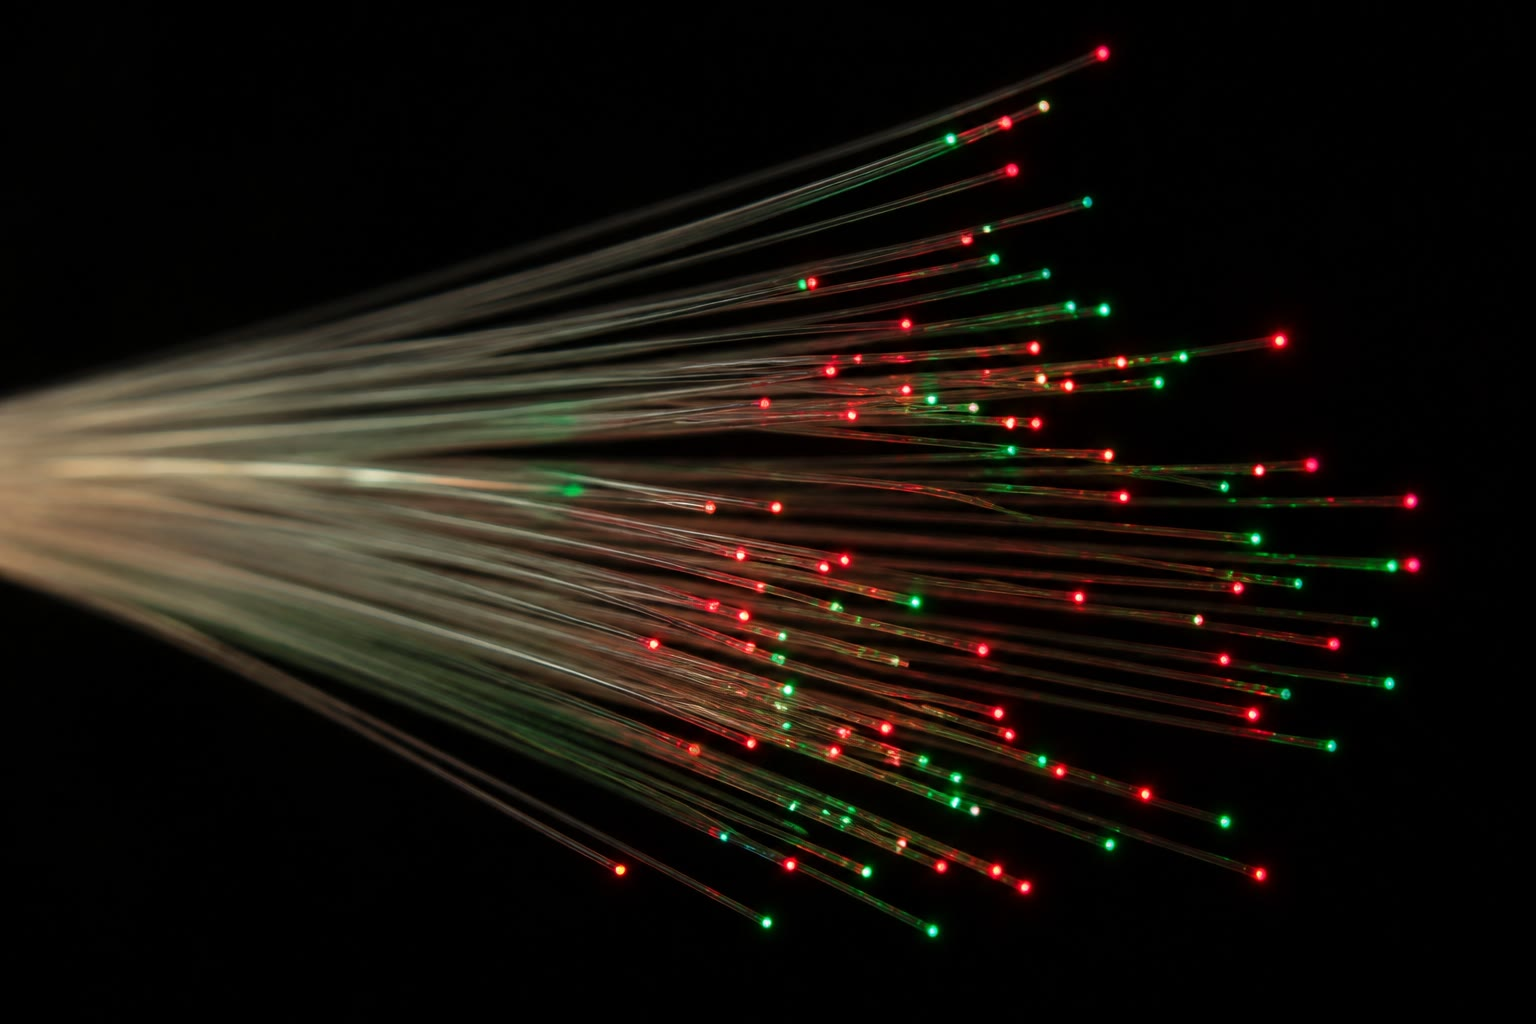
\includegraphics[width=0.58\linewidth]{images/book4/ai/b4-16-optical-fibres-glow.jpg}

{\small 从远端点亮的光纤：光借\omterm{thm:b2:wave-interfaces:snell}{全反射}被束缚在比头发丝还细的纤芯中，并沿每一处缓弯被导引。}
\end{omfigure}

\section{问题：烤箱谐振腔与光纤}

\begin{problem}[{周末问题——每个厨房与每座城市中的两类导波系统：
用驻波烹饪的烤箱，以及
承载互联网的光纤}]
\label{pb:b2:guided-waves:1}

\medskip
\noindent\textbf{第一部分——从磁控管到谐振腔。}
磁控管以 \qty{800}{W} 的功率、\qty{2.45}{GHz} 的频率，向一个矩形
波导（$a = \qty{8.6}{cm}$，$b = \qty{4.3}{cm}$）馈电，该波导通向
烤箱谐振腔（$30 \times 30 \times 20$ cm$^3$）；壁为钢制，$\gamma = \qty{1e6}{S/m}$。
\begin{enumerate}
  \item 求波导中 TE$_{10}$、TE$_{20}$、TE$_{01}$
        模式的截止频率；验证在 \qty{2.45}{GHz} 下只有 TE$_{10}$ 传播。
  \item 求 \qty{2.45}{GHz} 下波导的波长、\omterm{def:b2:dispersion-wave-packets:relation}{相速度}与\omterm{prop:b2:dispersion-wave-packets:group}{群速度}。
  \item 求 \qty{800}{W} 时波导中的场振幅 $E_0$（TE$_{10}$ 功率
        公式），并与空气的击穿场强比较。
  \item 宽壁上的表\omterm{prop:b2:maxwell-equations:boundary}{面电流}振幅（量级为
        $E_0/\mu_0c$），钢的\omterm{def:b2:dispersion-wave-packets:complex}{趋肤深度}与表面电阻；
        波导每米的损耗。
  \item 列出谐振腔中频率与
        \qty{2.45}{GHz} 相差在 $3\%$ 以内的模式（试取 $(m, n, p)$ 至 $4$）；有几个？
  \item 同类模式沿各轴向的热点间距；
        为何要转动转盘？何为“模式搅拌器”？
  \item 装有食物时谐振腔的品质因数约为
        $200$：求其响应带宽；为何磁控管频率与模式之间的
        失配影响不大。
  \item 空腔的 $Q \approx 3000$：\qty{800}{W} 输入功率下的储能、
        平均能量密度与场振幅；与
        第 3 题及击穿场强比较。什么保护磁控管，
        使其在烤箱空载运行时不受损？
  \item 求能量沿 \qty{20}{cm} 长的波导
        由磁控管传至谐振腔所需的时间。
  \item 磁控管由半波整流电源供电，仅在每个市电周期
        的一半时间内发射：求脉冲期间的峰值功率，
        已知其平均值为 \qty{800}{W}；
        脉冲间隔内谐振腔做什么？（取 $Q \approx 200$）
\end{enumerate}

\medskip
\noindent\textbf{部分 II——门与截止。}
\begin{enumerate}[resume]
  \item 门网上有 \qty{1.5}{mm} 的孔，板厚为 \qty{1}{mm}：求
        孔内的衰减长度，以及穿过金属板的衰减（以 dB 计）。
  \item 门的边缘由一个四分之一波长的“扼流器”封住：即一条环绕门框、
        深为 $\lambda/4$ 的缝隙，它在门框间隙处呈现断开的电路
        （回顾\cref{ch:b2:wave-interfaces}）：求
        \qty{2.45}{GHz} 下缝隙的深度。
  \item 法定泄漏量在 \qty{5}{cm} 处为 \qty{5}{mW/cm^2}：这相当于
        面积为 \qty{100}{cm^2} 的门通过的 \qty{800}{W} 功率的多大比例？
  \item 一根长 \qty{30}{cm}、直径 \qty{4}{cm} 的管道与谐振腔相通：它在
        \qty{2.45}{GHz} 下是否低于截止频率？求其长度上的衰减。
  \item 为何门网必须在门框四周与之电气相连
        （若连接处留有缺口，它会表现得像什么？）
\end{enumerate}

\medskip
\noindent\textbf{部分 III——光纤。}
阶跃折射率光纤：纤芯 $n_1 = 1.465$，包层 $n_2 = 1.460$，纤芯
直径为 \qty{50}{\micro m}（多模）或 \qty{9}{\micro m}（单模）；
$\lambda = \qty{1.55}{\micro m}$；衰减为 \qty{0.2}{dB/km}。
\begin{enumerate}[resume]
  \item 求\omterm{prop:b2:guided-waves:fibre}{数值孔径}与接收角；
        光是否容易耦合进入光纤？
  \item 求多模光纤每千米的模式展宽；最大
        比特率（在 \qty{10}{km} 上，每比特占一个展宽时间）。
  \item 求多模光纤的模式数（取 $N \approx
        \tfrac12(\pi d\,\mathrm{NA}/\lambda)^2$）；求单模光纤（$d =
        \qty{9}{\micro m}$）的模式数，验证同一公式给出约 $1$。
  \item 单模光纤中剩余的展宽来自色散：
        取 $\omega'' \approx \qty{-0.2}{m^2/s}$（见\cref{ch:b2:dispersion-wave-packets}），
        脉宽为 \qty{50}{ps} 的脉冲，求脉冲展宽一倍所经过的距离；
        求 \qty{100}{km} 上的比特率。
  \item 求 \qty{100}{km} 上的衰减，分别以 dB 和功率比表示；输入功率
        为 \qty{1}{mW}，求输出功率；若每隔 \qty{80}{km} 设一个放大器，
        则跨大西洋的 \qty{6000}{km} 链路需要多少个放大器？
  \item 求 \qty{1.55}{\micro m} 处的频率与光子能量；
        求功率为 \qty{1}{mW} 时每秒的光子数，以及在 \qty{10}{Gbit/s} 下每比特的光子数，
        分别计算输入端及经过 \qty{100}{km} 后的值。
  \item 为何取 \qty{1.55}{\micro m}（想一想石英的两种损耗：
        瑞利散射，按 $1/\lambda^4$ 下降；红外吸收，
        超过 \qty{1.6}{\micro m} 后上升）？
  \item 切割平整的光纤端面朝向空气时的菲涅耳反射，求以 dB 计的损耗；
        为何连接器采用折射率匹配凝胶，
        或抛光的物理接触？
  \item 光纤在平缓弯曲处为何不辐射，而在急弯处为何会漏光
        （想一想光线
        在纤芯边界上的入射角）？
  \item 比较本题的两种导波结构：何者约束波，
        何者限制带宽，两者的损耗又各由什么引起。
\end{enumerate}
\end{problem}
